\documentclass[9pt]{beamer}
\usepackage{beamerthemesplit}
%\usepackage{times}
\usepackage{graphicx}
\usepackage{algorithm}
\usepackage{algorithmic}
\usepackage{amsmath}
\usepackage{amssymb}
\usepackage{amsthm}
%\usepackage{thmtools,thm-restate}
\usepackage[font=small]{caption}
\usepackage{subcaption}
\usepackage{listings}
\usepackage{xcolor}
\usepackage{float}
\usepackage{animate}
\usepackage{media9}
\usepackage{multimedia}
\usepackage{hyperref}
\usepackage{cancel}

\usetheme{Madrid}

\graphicspath{{./images/}}

\AtBeginSection[]{
  \begin{frame}
  \vfill
  \centering
  \begin{beamercolorbox}[sep=8pt,center,shadow=true,rounded=true]{title}
    \usebeamerfont{title}\insertsectionhead\par%
  \end{beamercolorbox}
  \vfill
  \end{frame}
}


\newcommand{\underE}[2]{\underset{\begin{subarray}{c}#1 \end{subarray}}{\E}\left[ #2 \right]}


\newcommand\Fontvi{\fontsize{6}{7.2}\selectfont}
\renewcommand{\d}[1]{\ensuremath{\operatorname{d}\!{#1}}}

\newcommand{\twocolumns}[4]{
\begin{columns}
\begin{column}{#1\textwidth}
    #3
\end{column}
\begin{column}{#2\textwidth}
	#4
\end{column}
\end{columns}
}

\usepackage{listings}
\usepackage{color}
\usepackage{courier}
 
\definecolor{codegreen}{rgb}{0,0.6,0}
\definecolor{codegray}{rgb}{0.5,0.5,0.5}
\definecolor{codepurple}{rgb}{0.58,0,0.82}
\definecolor{backcolour}{rgb}{0.95,0.95,0.92}


\lstdefinestyle{mystyle}{
    backgroundcolor=\color{backcolour},   
    commentstyle=\color{codegreen},
    keywordstyle=\color{magenta},
    numberstyle=\tiny\color{codegray},
    stringstyle=\color{codepurple},
    basicstyle=\footnotesize\ttfamily,
    breakatwhitespace=false,         
    breaklines=true,                 
    captionpos=b,                    
    keepspaces=true,                 
    %numbers=left,                    
    numbersep=5pt,                  
    showspaces=false,                
    showstringspaces=false,
    showtabs=false,                  
    tabsize=2
}
 
\lstdefinestyle{mystyle2}{
    backgroundcolor=\color{backcolour},   
    commentstyle=\color{codegreen},
    keywordstyle=\color{magenta},
    numberstyle=\tiny\color{codegray},
    stringstyle=\color{codepurple},
    basicstyle=\tiny\ttfamily,
    breakatwhitespace=false,         
    breaklines=true,                 
    captionpos=b,                    
    keepspaces=true,                 
    %numbers=left,                    
    numbersep=5pt,                  
    showspaces=false,                
    showstringspaces=false,
    showtabs=false,                  
    tabsize=2
}

\lstdefinestyle{mystyle3}{
    backgroundcolor=\color{backcolour},   
    commentstyle=\color{codegreen},
    keywordstyle=\color{magenta},
    numberstyle=\tiny\color{codegray},
    stringstyle=\color{codepurple},
    basicstyle=\scriptsize\ttfamily,
    breakatwhitespace=false,         
    breaklines=true,                 
    captionpos=b,                    
    keepspaces=true,                 
    %numbers=left,                    
    numbersep=5pt,                  
    showspaces=false,                
    showstringspaces=false,
    showtabs=false,                  
    tabsize=2
}

\lstset{style=mystyle3}


\begin{document}
%
% Definitions and macros
%

%\setlength{\marginparwidth}{1.2in}
%\let\oldmarginpar\marginpar
%\renewcommand\marginpar[1]{\-\oldmarginpar[\raggedleft\footnotesize #1]%
%{\raggedright\footnotesize #1}}

%\renewcommand{\indexspace}{\rule{0cm}{.4cm}}
%% end example/remark
%\newcommand{\eex}{\ifmmode\sq\else{\unskip\nobreak\hfil
%  \penalty50\hskip1em\null\nobreak\hfil$\Diamond$
%  \parfillskip=0pt\finalhyphendemerits=0\endgraf}\fi{}}
%\newcommand{\erem}{\ifmmode\sq\else{\unskip\nobreak\hfil
%  \penalty50\hskip1em\null\nobreak\hfil$\star$
%  \parfillskip=0pt\finalhyphendemerits=0\endgraf}\fi{}}
%\newcommand{\eobs}{\ifmmode\sq\else{\unskip\nobreak\hfil
%  \penalty50\hskip1em\null\nobreak\hfil$\vartriangleleft$
%  \parfillskip=0pt\finalhyphendemerits=0\endgraf}\fi{}}

% VET - characters - lowercase
\newcommand{\avet}{{\mathbf  a}}
\newcommand{\bvet}{{\mathbf  b}}
\newcommand{\cvet}{{\mathbf  c}}
\newcommand{\dvet}{{\mathbf  d}}
\newcommand{\evet}{{\mathbf  e}}
\newcommand{\fvet}{{\mathbf  f}}
\newcommand{\gvet}{{\mathbf  g}}
\newcommand{\hvet}{{\mathbf  h}}
\newcommand{\ivet}{{\mathbf  i}}
\newcommand{\jvet}{{\mathbf  j}}
\newcommand{\kvet}{{\mathbf  k}}
\newcommand{\lvet}{{\mathbf  l}}
\newcommand{\mvet}{{\mathbf  m}}
\newcommand{\nvet}{{\mathbf  n}}
\newcommand{\ovet}{{\mathbf  o}}
\newcommand{\pvet}{{\mathbf  p}}
\newcommand{\qvet}{{\mathbf  q}}
\newcommand{\rvet}{{\mathbf  r}}
\newcommand{\svet}{{\mathbf  s}}
\newcommand{\tvet}{{\mathbf  t}}
\newcommand{\uvet}{{\mathbf  u}}
\newcommand{\vvet}{{\mathbf  v}}
\newcommand{\xvet}{{\mathbf  x}}
\newcommand{\yvet}{{\mathbf  y}}
\newcommand{\zvet}{{\mathbf  z}}
\newcommand{\wvet}{{\mathbf  w}}

% VET - characters - uppercase
\newcommand{\Avet}{{\mathbf  A}}
\newcommand{\Bvet}{{\mathbf  B}}
\newcommand{\Cvet}{{\mathbf  C}}
\newcommand{\Dvet}{{\mathbf  D}}
\newcommand{\Evet}{{\mathbf  E}}
\newcommand{\Fvet}{{\mathbf  F}}
\newcommand{\Gvet}{{\mathbf  G}}
\newcommand{\Hvet}{{\mathbf  H}}
\newcommand{\Ivet}{{\mathbf  I}}
\newcommand{\Jvet}{{\mathbf  J}}
\newcommand{\Kvet}{{\mathbf  K}}
\newcommand{\Lvet}{{\mathbf  L}}
\newcommand{\Mvet}{{\mathbf  M}}
\newcommand{\Nvet}{{\mathbf  N}}
\newcommand{\Ovet}{{\mathbf  O}}
\newcommand{\Pvet}{{\mathbf  P}}
\newcommand{\Qvet}{{\mathbf  Q}}
\newcommand{\Rvet}{{\mathbf  R}}
\newcommand{\Svet}{{\mathbf  S}}
\newcommand{\Tvet}{{\mathbf  T}}
\newcommand{\Uvet}{{\mathbf  U}}
\newcommand{\Xvet}{{\mathbf  X}}
\newcommand{\Yvet}{{\mathbf  Y}}
\newcommand{\Vvet}{{\mathbf  V}}
\newcommand{\Wvet}{{\mathbf  W}}
\newcommand{\Zvet}{{\mathbf  Z}}

\newcommand{\Deltavet}{\mathbf  \Delta}
\newcommand{\Lambdavet}{{\mathbf  \Lambda}}
\newcommand{\Sigmavet}{\mathbf  \Sigma}
\newcommand{\Thetavet}{{\mathbf  \Theta}}

% Special characters:
\newcommand{\s}{ {\sigma} }

\newcommand{\e}{{\mathrm e}}
\newcommand{\jm}{{\mathrm j}}
\newcommand{\E}{{\mathrm E}}
\newcommand{\Ex}{{\mathbb E}}
\renewcommand{\d}{{\mathrm d}}
\newcommand{\dt}{{\mathrm d}t}
\newcommand{\X}{ {\mathcal X} }
\newcommand{\Y}{ {\mathcal Y} }
\newcommand{\Z}{ {\mathcal Z} }



\newcommand{\calA}{{\mathcal A}}
\newcommand{\calB}{{\mathcal B}}
\newcommand{\calC}{{\mathcal C}}
\newcommand{\calD}{{\mathcal D}}
\newcommand{\calE}{{\mathcal E}}
\newcommand{\calF}{{\mathcal F}}
\newcommand{\calG}{{\mathcal G}}
\newcommand{\calH}{{\mathcal H}}
\newcommand{\calI}{{\mathcal I}}
\newcommand{\calJ}{{\mathcal J}}
\newcommand{\calK}{{\mathcal K}}
\newcommand{\calL}{{\mathcal L}}
\newcommand{\calM}{{\mathcal M}}
\newcommand{\calN}{{\mathcal N}}
\newcommand{\calO}{{\mathcal O}}
\newcommand{\calP}{{\mathcal P}}
\newcommand{\calQ}{{\mathcal Q}}
\newcommand{\calR}{{\mathcal R}}
\newcommand{\calS}{{\mathcal S}}
\newcommand{\calT}{{\mathcal T}}
\newcommand{\calU}{{\mathcal U}}
\newcommand{\calV}{{\mathcal V}}
\newcommand{\calX}{{\mathcal X}}
\newcommand{\calY}{{\mathcal Y}}
\newcommand{\calW}{{\mathcal W}}
\newcommand{\calZ}{{\mathcal Z}}
\newcommand{\qtil}{{\tilde{q}}}
\newcommand{\td}{{\tilde{\delta}}}

\newcommand{\vect}[1]{ {\mbox{\rm vec}(#1)} }

% Macro comandi:

\newcommand{\Atil}{\tilde{A}}
\newcommand{\Zhat}{\hat{Z}}
\newcommand{\Hbar}{\bar{H}}
\newcommand{\Dhat}{\hat{D}}
\newcommand{\dhat}{\hat{d}}
%

\newcommand{\rhat}{\hat{r}}
\newcommand{\xhat}{\hat{x}}
\newcommand{\yhat}{\hat{y}}
\newcommand{\zhat}{\hat{z}}
\newcommand{\xbar}{\bar{x}}
\newcommand{\ubar}{\bar{u}}
\newcommand{\ybar}{\bar{y}}
\newcommand{\zbar}{\bar{z}}
%
\newcommand{\pdot}{\dot{p}}
\newcommand{\pddot}{\ddot{p}}
\newcommand{\pbar}{\bar{p}}
%
\newcommand{\qdot}{\dot{q}}
\newcommand{\qddot}{\ddot{q}}
\newcommand{\qbar}{\bar{q}}
%
\newcommand{\xdot}{\dot{x}}
\newcommand{\ydot}{\dot{y}}
\newcommand{\zdot}{\dot{z}}
\newcommand{\yddot}{\ddot{y}}
\newcommand{\thdot}{\dot{\theta}}
\newcommand{\thddot}{\ddot{\theta}}
\newcommand{\util}{{\tilde{u}}}
\newcommand{\xtil}{{\tilde{x}}}
\newcommand{\ytil}{{\tilde{y}}}
\newcommand{\lam}{\lambda}
\newcommand{\lamax}{\lambda\ped{max}}
\newcommand{\lamin}{\lambda\ped{min}}
%
\newcommand{\adj}{ {\mbox{\rm adj}\;} }
\newcommand{\sign}{\mbox {\rm sgn}}
\newcommand{\spn}{\mbox {\rm span}}
\newcommand{\barJ}{\bar{J}}
\newcommand{\dom}{\mathop {\mathrm {dom}}}
\newcommand{\card}{\mathop{\mathrm{card}}}
\newcommand{\subt}{\mathop{\mathrm{s.t.}}}

\newcommand{\epi}{\mathop{\mathrm{epi}}}
\newcommand{\env}{\mathop{\mathrm{env}}}
\newcommand{\chull}{\mathop{\mathrm{co}}}
\newcommand{\graph}{\mathop{\mathrm{graph}}}
\newcommand{\prox}[1]{\mathop{\mathrm{prox}_{#1}}}
\newcommand{\sthr}[1]{\mathop{\mathrm{sthr}_{#1}}}

\def\hardsection{$\spadesuit\;$}





%%%% Fields and Groups
\newcommand{\Real}[1]{ { {\mathbb R}^{#1} } }
\newcommand{\Realp}[1]{ { {\mathbb R}_{+}^{#1} } }
\newcommand{\Realpp}[1]{ { {\mathbb R}_{++}^{#1} } }
\newcommand{\Complex}[1]{ { {\mathbb C}^{#1} } }
\newcommand{\Imag}[1]{ { {\mathbb I}^{#1} } }
\newcommand{\Field}[1]{ {\mathbb F}^{#1} }
\newcommand{\F}{ {\mathbb F}}
\newcommand{\Orth}[1]{ { {\calG_{\calO}^{#1}} } }
\newcommand{\Unit}[1]{ { {\calG_{\calU}^{#1}} } }
\newcommand{\Sym}[1]{ { {\mathbb S}^{#1} } }
\newcommand{\Symp}[1]{ { {\mathbb S}_{+}^{#1} } }
\newcommand{\Sympp}[1]{ { {\mathbb S}_{++}^{#1} } }
\newcommand{\Herm}[1]{ { {\mathbb H}^{#1} } }
\newcommand{\Skew}[1]{ { {\mathbb S\mathbb K}^{#1} } }
\newcommand{\Skherm}[1]{ { {\mathbb H\mathbb K}^{#1} } }
% manifolds (in matrices)
\newcommand{\Rman}[1]{ { {\mathcal R}^{#1} } } 
\newcommand{\Cman}[1]{ { {\mathcal C}^{#1} } }
%
\newcommand{\Hinf}[1]{ {  {\mathcal H}_\infty^{#1} } }
\newcommand{\RHinf}[1]{ { {\mathcal RH}_\infty^{#1} } }
\newcommand{\Htwo}[1]{ {  {\mathcal H}_2^{#1} } }
\newcommand{\RHtwo}[1]{ { {\mathcal RH}_2^{#1} } }

\newcommand{\dist}[1]{{\mathrm{dist}}{\left( #1 \right)}}
%
\newcommand{\diff}[2]{ \frac{\d {#1}}{\d {#2}}  }
\newcommand{\diffp}[2]{ \frac{\partial {#1}}{\partial {#2}}  }
\newcommand{\diffqd}[2]{ \frac{\d^2 {#1}}{\d {#2}^2}  }
\newcommand{\diffq}[2]{ \frac{\d^2 {#1}}{\d {#2}}  }
\newcommand{\diffqq}[3]{ \frac{\d^2 {#1}}{ \d {#2} \d {#3}  }}
\newcommand{\diffpq}[2]{ \frac{\partial^2 {#1}}{\partial {#2}^2}  }
\newcommand{\difftq}[3]{ \frac{\partial^2 {#1}}{\partial {#2}\partial {#3}}  }
\newcommand{\diffi}[3]{ \frac{\d^{#3} {#1}}{\d {#2}^{#3}}  }
\newcommand{\diffpi}[3]{ \frac{\partial^{#3} {#1}}{\partial {#2}^{#3}}  }
\newcommand{\binomial}[2]{\scriptsize{\left(\!\! \ba{c} #1 \\ #2 \ea \!\! \right)} }
\newcommand{\comb}[2]{{\left(\!\!\! \ba{c} #1 \\ #2 \ea \!\!\! \right)} }

\newcommand{\simax}{{\sigma_{\mathrm{max}}}}
\newcommand{\simin}{{\sigma_{\mathrm{min}}}}
\newcommand{\prob}{{\mbox{\rm Prob}}}
\newcommand{\var}{{\mbox{\rm var}}}
\newcommand{\sint}{{\mbox{\rm int}\,}} %set interior
\newcommand{\relint}{{\mbox{\rm relint}\,}} %set interior
\newcommand{\ns}{{\mbox{\tt ns}}} 

%

\newcommand{\rank}{\mathop{\mathrm{rank}}\nolimits}
\newcommand{\range}{\mathop{\mathcal{R}}\nolimits}
\newcommand{\nulsp}{\mathop{\mathcal{N}}\nolimits}
\newcommand{\diagop}{\mathop{\mathrm{diag}}\nolimits}
\newcommand{\Var}{\mathop{\mathrm{var}}\nolimits}
\newcommand{\tr}{\mathop{\mathrm{trace}}\nolimits}
\newcommand{\sinc}{\mathop{\mathrm{sinc}}\nolimits}

%%%% Real and Imaginary
\newcommand{\pre}[1]{ { {\mathop{\mathrm{Re}}}  \left({#1}\right)} }
\newcommand{\pim}[1]{ { {\mathop{\mathrm{Im}}}  ({#1})} }
\newcommand{\rp}{ ^{\Real{}} }
\newcommand{\ip}{ ^{\Imag{}} }



%%%% Various
\newcommand{\one}{{\mathbf  1}}
%\newcommand{\qed}{{\hfill $\square$}}
\newcommand{\dss}{\displaystyle}
\newcommand{\inv}{^{-1}}
\newcommand{\pinv}{^{\dagger}}
\newcommand{\diag}[1]{\mathrm{diag}\left({#1}\right)}
\newcommand{\blockdiag}[1]{\mbox{\rm bdiag}\left({#1}\right)}
\newcommand{\tran}{^{\top}}
\newcommand{\inner}[1]{\langle {#1} \rangle}
\newcommand{\ped}[1]{_{\mathrm{#1}}}
\newcommand{\ap}[1]{^{\mathrm{#1}}}

\newcommand{\blu}[1]{\textcolor{blue}{#1}}
\newcommand{\red}[1]{\textcolor{red}{#1}}
\newcommand{\green}[1]{\textcolor{green}{#1}}
\newcommand{\cyan}[1]{\textcolor{cyan}{#1}}
\newcommand{\comment}[1]{\vspace{.1cm} \blu{#1} \vspace{.1cm}}



%%%% Commands
\newcommand{\beq}{\begin{equation}}
\newcommand{\eeq}{\end{equation}}
\newcommand{\bea}{\begin{eqnarray}}
\newcommand{\eea}{\end{eqnarray}}
\newcommand{\beas}{\begin{eqnarray*}}
\newcommand{\eeas}{\end{eqnarray*}}
\newcommand{\ba}{\begin{array}}
\newcommand{\ea}{\end{array}}
\newcommand{\bit}{\begin{itemize}}
\newcommand{\eit}{\end{itemize}}
\newcommand{\ben}{\begin{enumerate}}
\newcommand{\een}{\end{enumerate}}
\newcommand{\bde}{\begin{description}}
\newcommand{\ede}{\end{description}}
\newcommand{\bsp}{\begin{split}}
\newcommand{\esp}{\end{split}}

%% Environments
%\newtheorem{corollary}{Corollary}
%\newtheorem{exercise}{Exercise}
%\newtheorem{solution}{Solution}
%\newtheorem{algorithm}{Algorithm}
%\newtheorem{assumption}{Assumption}
%\newtheorem{definition}{Definition}
%\newtheorem{proposition}{Proposition}
%\newtheorem{procedure}{Procedure}
%\newtheorem{lemma}{Lemma}
%\newtheorem{fact}{Fact}
%\newtheorem{example}{Example}
%\theoremstyle{remark}
%\newtheorem{theorem}{Theorem}
%\newtheorem*{remark}{Remark}

%%% margin stuff
%% example in the margin
%\newcommand{\marginex}[1]{
%\marginnote{\refstepcounter{examplectr}{\bfseries\textsf{Example \theexamplectr.}} 
%#1
%}}
%
%% remark in the margin
%\newcommand{\marginrmk}[1]{
%\marginnote{\refstepcounter{remarkctr}{\bfseries\textsf{Remark \theremarkctr.}} 
%#1
%}}
%
%% algorithm in the margin
%\newcommand{\marginalg}[1]{
%\marginnote{\refstepcounter{algorithmctr}{\bfseries\textsf{Algorithm \thealgorithmctr.}} 
%#1
%}}

%% misc
% these commands are to make things compile
\def\nocolon{}

% Prints the month name (e.g., January) and the year (e.g., 2008)
\newcommand{\monthyear}{%
  \ifcase\month\or January\or February\or March\or April\or May\or June\or
  July\or August\or September\or October\or November\or
  December\fi\space\number\year
}

% Prints an epigraph and speaker in sans serif, all-caps type.
\newcommand{\openepigraph}[2]{%
  %\sffamily\fontsize{14}{16}\selectfont
  \begin{fullwidth}
  \sffamily\large
  \begin{doublespace}
  \noindent\allcaps{#1}\\% epigraph
  \noindent\allcaps{#2}% author
  \end{doublespace}
  \end{fullwidth}
}

% Inserts a blank page
\newcommand{\blankpage}{\newpage\hbox{}\thispagestyle{empty}\newpage}




\title{Introduction to Deep RL, Part 1}
\author{Joshua Achiam}
\institute{OpenAI}
\titlegraphic{\includegraphics[height=2cm]{spinning-up-logo2}}
%\date{March 3, 2018}

\begin{frame}
\titlepage
\end{frame}


\section{1.0: What is Spinning Up?}

\begin{frame}{Education at OpenAI}

Mandate from OpenAI Charter: 
\begin{itemize}
\item "We seek to create a global community working together to address AGI’s global challenges."
\item "We are committed to providing public goods that help society navigate the path to AGI."
\end{itemize}
\begin{figure}
\centering
\includegraphics[height=5cm]{education_at_openai}
\end{figure}

\begin{center}
\url{https://blog.openai.com/openai-charter/}
\end{center}
\end{frame}

\begin{frame}{Spinning Up in Deep RL}

Deep RL will be a key technology in AGI: therefore, it is important to educate the public.
\begin{columns}
\begin{column}{0.5\textwidth}
\begin{figure}
\centering
\includegraphics[height=5cm]{spinningup_website}
\end{figure}
\end{column}
\begin{column}{0.5\textwidth}
\begin{itemize}
\item A short intro to RL 
\item An essay about becoming an RL researcher
\item A curated list of important papers
\item A code repo of key algorithms (VPG, TRPO, PPO, DDPG, TD3, SAC)
\item Warm-up coding exercises
\end{itemize}
\end{column}
\end{columns}
\begin{center}
\url{https://spinningup.openai.com/en/latest/}
\end{center}

\end{frame}

\begin{frame}{Spinning Up Workshops}

Hypothesis:
\begin{itemize}
\item Working with people directly will help them learn and build skills faster
\end{itemize}

Educational objectives:
\begin{itemize}
\item Teach current capabilities and limitations of deep RL
\item Raise awareness of work that needs doing in the field
\item Participants run and tinker with deep RL algorithms for the first time, and feel confident that they can keep doing it
\end{itemize}
\begin{figure}
\centering
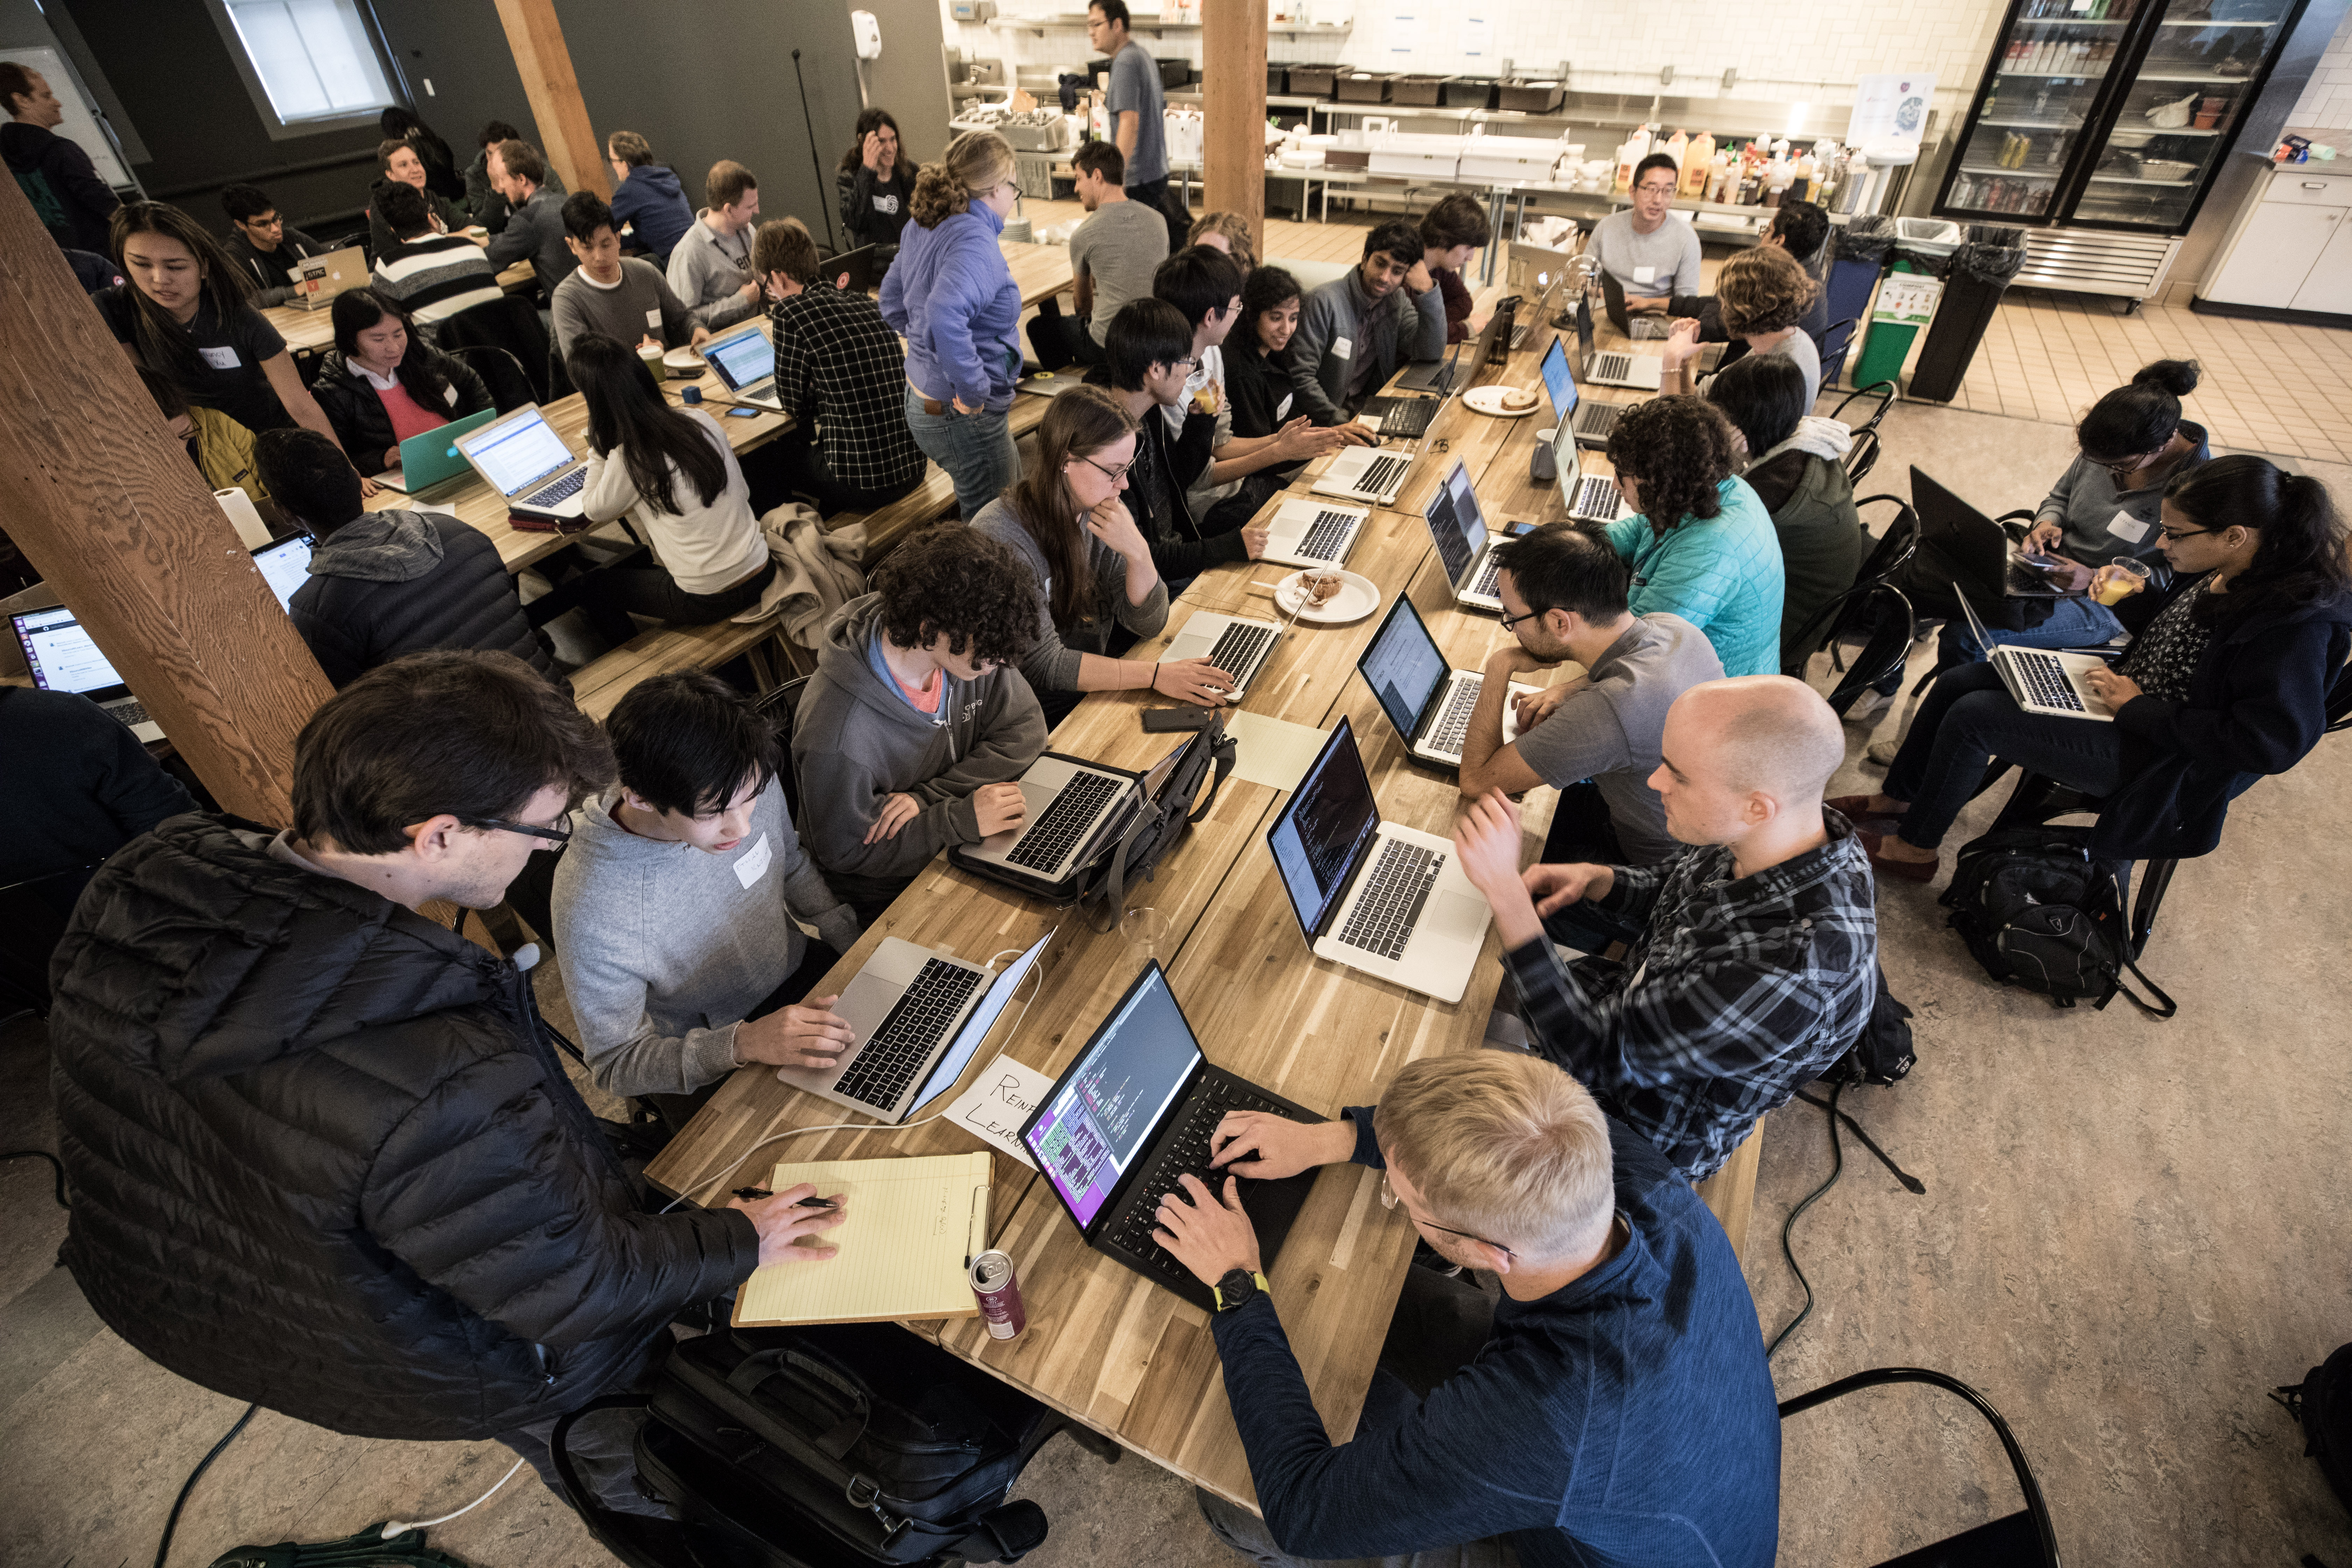
\includegraphics[height=3cm]{hackathon}
\end{figure}

\end{frame}

\section{1.1: What is deep RL, and why do we need it?}


\begin{frame}{What is Deep RL?}
Deep RL is the combination of \textbf{reinforcement learning (RL)} with \textbf{deep learning}

\begin{itemize}
\item \textbf{Reinforcement learning} is about solving problems by \textbf{trial and error}
\item \textbf{Deep learning} is about using \textbf{deep neural networks} to solve problems
\item $\Longrightarrow$ \textbf{Deep reinforcement learning} trains deep neural networks with trial and error
\end{itemize}

\twocolumns{0.4}{0.6}{
\begin{figure}
\centering
\includegraphics[width=\textwidth]{deep-neural-networks}
\end{figure}
}{
\begin{figure}
\centering
\includegraphics[width=\textwidth]{agent-interaction-loop}
\end{figure}
}
\begin{center}
Deep neural network\footnote{Deep neural network image from Gary Marcus} and RL interaction loop
\end{center}
\end{frame}

\begin{frame}{When would you want to use RL?}

RL is useful when
%
\begin{itemize}
\item you have a sequential decision-making problem
\item you do \textbf{not} know the optimal behavior already\footnotemark[1]
\item but you can still evaluate whether behaviors are good or bad
\end{itemize}

\vspace{3em}

That is, 

\begin{center}
\boxed{
\textbf{RL is useful when evaluating behaviors is easier than generating them}
}
\end{center}

\footnotetext[1]{Critical difference from supervised learning!}

\end{frame}

\begin{frame}{When would you want to use deep learning?}

\twocolumns{0.5}{0.5}{
Deep learning is useful when
%
\begin{itemize}
\item you want to approximate a function
\item function requires ``intelligence"
\item inputs and/or outputs are high-dimensional
\item lots of data is available
\end{itemize}

\vspace{2em}

This includes \textbf{tons} of problems!
%
\begin{itemize}
\item image recognition / facial classification
\item sentiment analysis
\item neural machine translation
\item automatic speech recognition
\item etc.
\end{itemize}
}{
\begin{figure}
\centering
\includegraphics[width=0.85\textwidth]{dl-object-detection}
\caption{Object detection\footnotemark[1]}
\end{figure}
\begin{figure}
\includegraphics[width=0.85\textwidth]{dl-neural-machine-translation}
\caption{Machine translation\footnotemark[2]}
\end{figure}
}

\footnotetext[1]{Intel Software,``A Closer Look at Object Detection, Recognition and Tracking"}
\footnotetext[2]{Nvidia Developer Blog, ``Introduction to Neural Machine Translation with GPUs"}

\end{frame}

\begin{frame}{When would you want to use deep RL?}
Deep RL can...
\begin{itemize}
\item Play video games from raw pixels
\item Control robots in simulation and in the real world
\item Play Go, Dota, and Starcraft at superhuman levels
\end{itemize}

\begin{columns}
\begin{column}{0.33\textwidth}
    \begin{center}
     \includegraphics[width=0.9\textwidth]{ms_pacman}

     \includegraphics[width=0.9\textwidth]{alphago}
     \end{center}
\end{column}
\begin{column}{0.67\textwidth}
\movie[width=0.9\textwidth, autostart, loop]{\includegraphics[width=0.9\textwidth]{knocked_down_standup}}{images/knocked-over-stand-up.mp4}
\end{column}
\end{columns}
\end{frame}

\section{Interlude: Recap of deep learning patterns}

\begin{frame}{Deep Learning: High-level}

Usual paradigm:
%
\begin{itemize}
\item we want to find a \textbf{model} that gives target \textbf{outputs} for particular \textbf{inputs},
\item we represent the model as a \textbf{function of parameters},
\begin{equation*}
f_{\theta}(x) = W_2 \sigma\left( W_1 x + b_1 \right) + b_2, \;\;\;\;\; \theta = \{W_1, W_2, b_1, b_2\}
\end{equation*}
\item we can evaluate the model performance with a \textbf{differentiable loss function} that depends on \textbf{a set of data},
\begin{equation*}
\calL(\theta) = \frac{1}{|\calD|}\sum_{(x,y)\in\calD} L(x,y,f_{\theta}(x))
\end{equation*}
\item and we find the optimal model by \textbf{gradient descent on the loss}.
\begin{equation*}
\theta \leftarrow \theta - \alpha \nabla_{\theta} \calL(\theta)
\end{equation*}
\end{itemize}

\end{frame}

\begin{frame}{Deep Learning: What makes it deep?}

\begin{itemize}
\item ``Deep" refers to using \textbf{function composition} as the building block for models

\item Deep models have many \textbf{layers}: output of one layer is input to next
\end{itemize}


\twocolumns{0.5}{0.5}{
\begin{figure}
\centering
\includegraphics[width=0.8\textwidth]{deep-neural-networks}
\end{figure}
\begin{figure}
\centering
\includegraphics[width=0.8\textwidth]{dl-colah-lstm}
\end{figure}
}{
\begin{figure}
\centering
\includegraphics[height=6cm]{dl-transformer}
\end{figure}
}

\footnotetext[1]{MLP credit: Gary Marcus, LSTM credit: Chris Olah, Transformer credit: Vaswani et al 2017}
\end{frame}

\begin{frame}{Deep Learning: What else?}

\begin{itemize}
\item Regularizers make optimization problems better-behaved:
\begin{equation*}
\calL(\theta) \to \calL(\theta) + \lambda \Omega(\theta)
\end{equation*}
\item Normalization makes optimization easier:
\begin{equation*}
a \to \frac{g}{\sigma}\left(a - \mu\right) + b
\end{equation*}
\item Adaptive optimizers (eg Adam) makes optimization faster:
\begin{align*}
m &\leftarrow \beta_1 m + (1-\beta_1) g \\
v &\leftarrow \beta_2 v + (1-\beta_2) g^2 \\
\theta &\leftarrow \theta - \alpha \frac{m}{\sqrt{v}+\epsilon}
\end{align*}
\item Reparameterization trick comes in handy sometimes:
%
\begin{equation*}
\underE{x \sim p_{\theta}}{F(x)} = \underE{z \sim \calN}{F(\xi(\theta, z))}
\end{equation*}
\item For links to detailed resources, see the Spinning Up essay!
\end{itemize}

\end{frame}

\section{1.2: How do we formulate RL problems?}


\begin{frame}[fragile]{What is RL?}

\begin{itemize}
\item An \textit{agent} interacts with an \textit{environment}. 
\begin{columns}
\begin{column}{0.5\textwidth}
    \begin{center}
     \includegraphics[width=\textwidth]{rl_diagram}
     \end{center}
\end{column}
\begin{column}{0.5\textwidth}  %%<--- here
\begin{lstlisting}[language=python]
  obs = env.reset()
  done = False
  while not(done):
  	act = agent.get_action(obs)
  	next_obs, reward, done, info = env.step(act)
  	obs = next_obs
\end{lstlisting}
\end{column}
\end{columns}
\item The goal of the agent is to maximize cumulative reward (called \textit{return}). 
\item The agent figures out how to attain its goal by trial and error.
\item Reinforcement learning (RL) is a field of study for algorithms that do that.
\end{itemize}

\end{frame}


\begin{frame}{Key Concepts in RL}

Before we can talk about algorithms, we have to talk about:
\begin{itemize}
\item Observation and action spaces
\item Policies
\item Trajectories
\item Reward and return
\item The RL optimization problem
\item Value and Action-Value Functions
\end{itemize}

\end{frame}

\begin{frame}{Observation and action spaces}

\begin{itemize}
\item A \textbf{state} is a complete-information description of the world
\item An \textbf{observation} is what the agent sees about the current state of the world
\item An environment is \textbf{fully observed} if the agent observes the whole state, otherwise \textbf{partially observed}
\item States, observations, and \textbf{actions} may be \textbf{continuous} or \textbf{discrete}
\end{itemize}

\begin{columns}
\begin{column}{0.5\textwidth}
\begin{center}
\includegraphics[width=0.9\textwidth]{ms_pacman}

Partially observed, continuous observation, discrete action
\end{center}
\end{column}
\begin{column}{0.5\textwidth}
\begin{center}
\includegraphics[width=0.9\textwidth]{knocked_down_standup}

Fully observed, continuous observation, continous action
\end{center}

\end{column}
\end{columns}

\end{frame}

\begin{frame}[fragile]{Policies}

A \textbf{policy} $\pi$ is a rule for selecting actions. It can be either
\begin{itemize}
\item \textbf{stochastic}, which means that it gives a probability distribution over actions, and actions are selected randomly based on that distribution ($a_t \sim \pi(\cdot|s_t)$),
\item or \textbf{deterministic}, which means that $\pi$ directly maps to an action ($a_t = \pi(s_t)$). 
\end{itemize}

\pause


\lstset{style=mystyle}

Examples of policies:
%
\begin{itemize}
\item Stochastic policy over discrete actions:
\begin{lstlisting}[language=python]
  obs = tf.placeholder(shape=(None, obs_dim), dtype=tf.float32)
  net = mlp(obs, hidden_dims=(64,64), activation=tf.tanh)
  logits = tf.layers.dense(net, units=num_actions, activation=None)
  actions = tf.squeeze(tf.multinomial(logits=logits,num_samples=1), axis=1)
\end{lstlisting}
\item Deterministic policy for a vector-valued continuous action:
\begin{lstlisting}[language=python]
  obs = tf.placeholder(shape=(None, obs_dim), dtype=tf.float32)
  net = mlp(obs, hidden_dims=(64,64), activation=tf.tanh)
  actions = tf.layers.dense(net, units=act_dim, activation=None)
\end{lstlisting}

\end{itemize}

\lstset{style=mystyle3}

\end{frame}


\begin{frame}{Trajectories}

\begin{itemize}
\item A \textbf{trajectory} $\tau$ is a sequence of states and actions in an environment:
\begin{equation*}
\tau = (s_0, a_0, s_1, a_1, ...).
\end{equation*}
\begin{itemize}
\item The initial state $s_0$ is sampled from a \textit{start state distribution} $\mu$:
%
\begin{equation*}
s_0 \sim \mu(\cdot).
\end{equation*}
\item State transitions depend only on the most recent state and action. They could be deterministic:
%
\begin{equation*}
s_{t+1} = f(s_t, a_t),
\end{equation*}
%
or stochastic:
%
\begin{equation*}
s_{t+1} \sim P(\cdot | s_t, a_t).
\end{equation*}
\end{itemize}
\item A trajectory is sometimes also called an \textbf{episode} or \textbf{rollout}. 
\end{itemize}

\end{frame}


\begin{frame}{Reward and Return}

The \textbf{reward} function of an environment measures how good state-action pairs are:
%
\begin{equation*}
r_t = R(s_t, a_t).
\end{equation*}

\begin{itemize}
\item Example: if you want a robot to run forwards but use minimal energy, $R(s, a) = v - \alpha \|a\|_2^2$. 
\end{itemize}
\pause
The \textbf{return} of a trajectory is a measure of cumulative reward along it. There are two main ways to compute return:
\begin{itemize}
\item Finite horizon undiscounted sum of rewards::
\begin{equation*}
R(\tau) = \sum_{t=0}^T r_t
\end{equation*}
\item Infinite horizon discounted sum of rewards:
\begin{equation*}
R(\tau) = \sum_{t=0}^{\infty} \gamma^t r_t
\end{equation*}
%
where $\gamma \in (0,1)$. This makes rewards less valuable if they are further in the future. (Why would we ever want this? Think about cash: it's valuable to have it sooner rather than later!)
\end{itemize}

\end{frame}

\begin{frame}{Reward-to-Go}

A closely-related quantity is \textbf{reward-to-go}, which is ``return starting from a state or timestep":
%
\begin{equation*}
R_t = \sum_{t'=t}^T r_{t'}
\end{equation*}
%
or
\begin{equation*}
R_t = \sum_{t'=t}^{\infty} \gamma^{t'-t} r_{t'}
\end{equation*}
\end{frame}

\begin{frame}{The Reinforcement Learning Problem}

In RL we want a policy which maximizes expected return. Thus the performance measure is
%
\begin{equation*}
J(\pi) = \underE{\tau \sim \pi}{R(\tau)},
\end{equation*}
%
and the \textbf{optimal policy} $\pi^*$ is:
%
\begin{equation*}
\pi^* = \arg \max_{\pi} J(\pi)
\end{equation*}

Note that by $\tau \sim \pi$, we mean
%
\begin{equation*}
s_0 \sim \mu(\cdot), \;\;\;\;\; a_t \sim \pi(\cdot|s_t), \;\;\;\;\; s_{t+1} \sim P(\cdot | s_t, a_t).
\end{equation*}

\end{frame}


\begin{frame}{Value Functions, Action-Value Functions, and Advantage Functions}

Value and action-value functions tell you the expected return after a state or state-action pair.
%
\begin{align*}
V^{\pi}(s) &= \underE{\tau \sim \pi}{R(\tau)\left| s_0 = s\right.} && \text{Start in }s\text{ and then sample from }\pi \\
Q^{\pi}(s,a) &= \underE{\tau \sim \pi}{R(\tau)\left| s_0 = s, a_0 = a\right.} && \text{Start in }s\text{, take action }a\text{, then sample from }\pi \\
V^*(s) &= \max_{\pi} \underE{\tau \sim \pi}{R(\tau)\left| s_0 = s\right.} && \text{Start in }s\text{ and then act optimally} \\
Q^*(s,a) &= \max_{\pi} \underE{\tau \sim \pi}{R(\tau)\left| s_0 = s, a_0 = a\right.} &&\text{Start in }s\text{, take action }a\text{, then act optimally}
\end{align*}

Value and action-value functions are connected:
%
\begin{align*}
V^{\pi}(s) &= \underE{a \sim \pi}{Q^{\pi}(s,a)}
\end{align*}

The advantage function for a policy tells you how much better or worse one action is than average:
%
\begin{align*}
A^{\pi}(s,a) &= Q^{\pi}(s,a) - V^{\pi}(s) 
\end{align*}

\end{frame}

\begin{frame}{Bellman Equations}

The value functions satisfy recursive \textbf{Bellman equations}:
%
\begin{align*}
V^{\pi}(s) &= \underE{a \sim \pi \\ s'\sim P}{r(s,a) + \gamma V^{\pi}(s')} \\
V^*(s) &= \max_a \underE{s'\sim P}{r(s,a) + \gamma V^*(s')} \\
Q^{\pi}(s,a) &= \underE{s'\sim P}{r(s,a) + \gamma \underE{a'\sim \pi}{Q^{\pi}(s',a')}} \\
Q^*(s,a) &= \underE{s'\sim P}{r(s,a) + \gamma \max_{a'} Q^*(s',a')}
\end{align*}

Basic idea: \textbf{The value of your starting point is the reward you expect to get from being there, plus the (discounted) value of wherever you land next.}

\vspace{2em}

Put another way: the cash you make in the rest of your life is the cash you make today plus all the cash you make for the rest of your life starting tomorrow

\end{frame}

%\begin{frame}{Operator Form of Bellman Equations}
%
%In operator form, where $\calT_v : V \to V$ and $\calT_q: Q\to Q$,
%%
%\begin{align*}
%V^{\pi} &= \calT^{\pi}_v V^{\pi} \\
%V^* &= \calT^*_v V^* \\
%Q^{\pi} &= \calT^{\pi}_q Q^{\pi} \\
%Q^* &= \calT^*_q Q^*
%\end{align*}
%\end{frame}

\begin{frame}{$Q^*$}
The optimal $Q$ function, $Q^*$, is especially important because it gives us a policy. In any state $s$, the optimal action is
%
\begin{equation*}
a^* = \arg \max_a Q^* (s, a).
\end{equation*}

We can measure how good a $Q^*$-approximator, $Q_{\theta}$, is by measuring its \textbf{mean-squared Bellman error}:
%
\begin{equation*}
\ell(\theta) = \frac{1}{|\calD|} \sum_{(s,a,s',r) \in \calD} \left( Q_{\theta}(s,a) - \left(r + \gamma \max_{a'} Q_{\theta}(s',a')\right)\right)^2.
\end{equation*}
%
This (roughly) says how well it satisfies the Bellman equation
%
\begin{equation*}
Q^*(s,a) = \underE{s'\sim P}{r(s,a) + \gamma \max_{a'} Q^* (s',a')}
\end{equation*}

\end{frame}

\section{1.3: What kinds of RL algorithms are there?}

\begin{frame}{Deep RL Algorithms}
There are many different kinds of RL algorithms! This is a non-exhaustive taxonomy (with specific algorithms in blue):
\begin{figure}
\centering
\includegraphics[width=\linewidth]{rl_algorithms_9_15}
\end{figure}
\end{frame}

\begin{frame}{Alphabet soup aside---what are they doing?}


\begin{columns}
\begin{column}{0.33\textwidth}
\includegraphics[width=0.9\textwidth]{rl_loop}
\end{column}
\begin{column}{0.67\textwidth}
Key steps in all RL algorithms:
\begin{itemize}
\item Run policy: actually act in env
\item Evaluate policy: estimate $V^{\pi}$ or $Q^*$
\item Improve policy: do something which lets you pick better actions
\end{itemize}

Major design decisions:
\begin{itemize}
\item Use a model of the env or not (can slot into any of those three steps)
\item Optimize stochastic policy directly or learn $Q^*$ as main controller
\end{itemize}
\end{column}
\end{columns}

\end{frame}

\begin{frame}{Model-Free RL: Policy Optimization}
\begin{figure}
\centering
\includegraphics[width=\linewidth]{rl_algorithms_polopt_only}
\end{figure}
\end{frame}

\begin{frame}{Model-Free RL: Policy Optimization}


\begin{columns}
\begin{column}{0.33\textwidth}
\includegraphics[width=0.9\textwidth]{rl_loop}
\end{column}
\begin{column}{0.67\textwidth}
\textbf{Policy Optimization}
\begin{itemize}
\item Run policy: Collect trajectories $\tau \sim \pi_{\theta}$
\item Evaluate policy: Estimate $V^{\pi_{\theta}}$, $A^{\pi_{\theta}}$ using current trajectories (\textbf{on-policy})
\item Improve policy: Increase likelihood of actions with high advantage
\end{itemize}
\end{column}
\end{columns}
\end{frame}

\begin{frame}{Warning: Math}

\begin{figure}
\centering
\includegraphics[width=4cm]{palpatine}
\end{figure}

\end{frame}

\begin{frame}{Wait, but why?}


\textbf{Deep RL is not mature enough to be a black box yet: you need to know some of this stuff to work with it successfully.}

\end{frame}

\begin{frame}{Mathematical Foundations of Policy Optimization}

In policy optimization, we train a \textbf{stochastic policy} $\pi_{\theta}$, usually in an \textbf{on-policy way}, to \textbf{maximize performance} $J(\pi_{\theta})$.

\vspace{1em}

What we'll cover:
\begin{itemize}
\item Direct gradient ascent on $J(\pi_{\theta})$ (VPG)
\item Various formulations of $\nabla_{\theta} J(\pi_{\theta})$
\item Some material about natural policy gradients
\end{itemize}

\end{frame}

\begin{frame}{The Policy Gradient}

Goal: derive an expression for $\nabla_{\theta} J(\pi_{\theta})$ which we can compute with a sample estimate, as the basis for a direct gradient ascent algorithm
%
\begin{equation*}
\theta \leftarrow \theta + \alpha \nabla_{\theta} J(\pi_{\theta})
\end{equation*}

\pause
\vspace{1em}

Well what happens if we just...
%
\begin{align*}
\nabla_{\theta} J(\pi_{\theta}) &= \nabla_{\theta} \underE{\tau \sim \pi_{\theta}}{R(\tau)}
\end{align*}

Problem: parameters are in distribution!

\end{frame}

\begin{frame}{The Policy Gradient: First Steps}

Solution: expand expectation into integral, use log-derivative trick
%
\begin{align*}
\nabla_{\theta} J(\pi_{\theta}) &= \nabla_{\theta} \underE{\tau \sim \pi_{\theta}}{R(\tau)} \\
&= \nabla_{\theta} \int d\tau P(\tau | \pi_{\theta}) R(\tau) \\
&= \int d\tau \nabla_{\theta} P(\tau | \pi_{\theta}) R(\tau) \\
&= \int d\tau {\color{red} P(\tau | \pi_{\theta}) \nabla_{\theta} \log P(\tau | \pi_{\theta})} R(\tau) \\
&= \underE{\tau \sim \pi_{\theta}}{\nabla_{\theta} \log P(\tau | \pi_{\theta}) R(\tau) }
\end{align*}

But are we done yet? No! Still need to compute $\nabla_{\theta} \log P(\tau | \pi_{\theta})$

\end{frame}

\begin{frame}{The Policy Gradient: Gradient of Trajectory Distribution}

What is $P(\tau|\pi_{\theta})$?
%
\begin{equation*}
P(\tau | \pi_{\theta}) = \mu(s_0) \prod_{t=0}^T P(s_{t+1} | s_t, a_t) \pi_{\theta}(a_t |s_t)
\end{equation*}

Thus:
%
\begin{align*}
\nabla_{\theta} \log P(\tau|\pi_{\theta}) &= \nabla_{\theta} \log \left(\mu(s_0) \prod_{t=0}^T P(s_{t+1} | s_t, a_t) \pi_{\theta}(a_t |s_t)\right) \\
&= \nabla_{\theta} \left(\log \mu(s_0) + \sum_{t=0}^T \left(\log P(s_{t+1} | s_t, a_t) + \log \pi_{\theta}(a_t |s_t) \right)\right) \\
&= \nabla_{\theta} \log \mu(s_0) + \sum_{t=0}^T \left(\nabla_{\theta} \log P(s_{t+1} | s_t, a_t) + \nabla_{\theta} \log \pi_{\theta}(a_t |s_t) \right) \\
&= {\color{red}\cancel{\nabla_{\theta} \log \mu(s_0)}} + \sum_{t=0}^T \left({\color{red}\cancel{\nabla_{\theta} \log P(s_{t+1} | s_t, a_t)}} + \nabla_{\theta} \log \pi_{\theta}(a_t |s_t) \right) \\
\therefore \nabla_{\theta} \log P(\tau|\pi_{\theta}) &= \sum_{t=0}^T \nabla_{\theta} \log \pi_{\theta}(a_t | s_t)
\end{align*}

\end{frame}

\begin{frame}{The Policy Gradient: So Far}
Putting it all together so far:
%
\begin{equation*}
\nabla_{\theta} J(\pi_{\theta}) = \underE{\tau \sim \pi_{\theta}}{\sum_{t=0}^T \nabla_{\theta} \log \pi_{\theta}(a_t | s_t) R(\tau)}
\end{equation*}

So we could estimate with:
%
\begin{align*}
\nabla_{\theta} J(\pi_{\theta}) &\approx \frac{1}{|\calD|} \sum_{\tau \in\calD} \sum_{t=0}^T \nabla_{\theta} \log \pi_{\theta}(a_t | s_t) R(\tau)
\end{align*}

But not good enough! Variance will be high.

\end{frame}

\begin{frame}{The Policy Gradient: Variance Reduction}

Insight: future actions and past rewards should be uncorrelated. That is:
%
\begin{equation*}
\text{for } t > t', \;\;\; \E\left[\nabla_{\theta} \log \pi_{\theta}(a_t | s_t) r_{t'}\right] = 0
\end{equation*}

Thus:
%
\begin{align*}
\nabla_{\theta} J(\pi_{\theta}) &= \underE{\tau \sim \pi_{\theta}}{\sum_{t=0}^T \nabla_{\theta} \log \pi_{\theta}(a_t | s_t) R(\tau)} \\
&= \underE{\tau \sim \pi_{\theta}}{\sum_{t=0}^T \nabla_{\theta} \log \pi_{\theta}(a_t | s_t) \sum_{t'=0}^T r_{t'}} \\
&= \sum_{t=0}^T \sum_{t'=0}^T \underE{\tau \sim \pi_{\theta}}{\nabla_{\theta} \log \pi_{\theta}(a_t | s_t)r_{t'}} \\
&= \sum_{t=0}^T \sum_{{\color{red}t'=t}}^T\underE{\tau \sim \pi_{\theta}}{\nabla_{\theta} \log \pi_{\theta}(a_t | s_t)r_{t'}} \\
\therefore \nabla_{\theta} J(\pi_{\theta}) &= \underE{\tau \sim \pi_{\theta}}{\sum_{t=0}^T \nabla_{\theta} \log \pi_{\theta}(a_t | s_t) \sum_{t'=t}^T r_{t'}} 
\end{align*}

\end{frame}

\begin{frame}{The Policy Gradient: Alternate Forms}

What we have currently: ``Reward-to-Go" policy gradient:
%
\begin{equation*}
\nabla_{\theta} J(\pi_{\theta}) = \underE{\tau \sim \pi_{\theta}}{\sum_{t=0}^T \nabla_{\theta} \log \pi_{\theta}(a_t | s_t) \sum_{t'=t}^T r_{t'}} 
\end{equation*}

Observe: expectation can be broken up, letting us transform ``Reward-to-Go" into $Q^{\pi}$:
%
\begin{align*}
\nabla_{\theta} J(\pi_{\theta}) &= \underE{\tau \sim \pi_{\theta}}{\sum_{t=0}^T \nabla_{\theta} \log \pi_{\theta}(a_t | s_t) \sum_{t'=t}^T r_{t'}} \\
&= \sum_{t=0}^T \underE{\tau \sim \pi_{\theta}}{\nabla_{\theta} \log \pi_{\theta}(a_t | s_t) \sum_{t'=t}^T r_{t'}} \\
&= \sum_{t=0}^T \underE{\tau_{0:t} \sim \pi_{\theta}}{\nabla_{\theta} \log \pi_{\theta}(a_t | s_t) \underE{\tau_{(t+1):T} \sim \pi_{\theta}}{\sum_{t'=t}^T r_{t'}}} \\
&= \sum_{t=0}^T \underE{\tau_{0:t} \sim \pi_{\theta}}{\nabla_{\theta} \log \pi_{\theta}(a_t | s_t) Q^{\pi_{\theta}}(s_t, a_t)} \\
\therefore \nabla_{\theta} J(\pi_{\theta}) &=\underE{\tau \sim \pi_{\theta}}{\sum_{t=0}^T \nabla_{\theta} \log \pi_{\theta}(a_t | s_t) Q^{\pi_{\theta}}(s_t, a_t)}
\end{align*}

\end{frame}

\begin{frame}{The Policy Gradient: Baselines}

What is a \textbf{baseline}? A function $b(s_t)$ with
%
\begin{equation*}
\nabla_{\theta} J(\pi_{\theta}) =\underE{\tau \sim \pi_{\theta}}{\sum_{t=0}^T \nabla_{\theta} \log \pi_{\theta}(a_t | s_t) \left(Q^{\pi_{\theta}}(s_t, a_t) - b(s_t)\right)}
\end{equation*}
%
Claim: this works for any $b$! Proof:
%
\begin{align*}
\underE{a_t \sim \pi_{\theta}(\cdot|s_t)}{\nabla_{\theta} \log \pi_{\theta}(a_t | s_t) b(s_t)} &= \underE{a_t \sim \pi_{\theta}(\cdot|s_t)}{\nabla_{\theta} \log \pi_{\theta}(a_t | s_t)} b(s_t) \\
&= \left(\int da \pi_{\theta}(a_t|s_t) \nabla_{\theta} \log \pi_{\theta}(a_t|s_t)\right) b(s_t) \\
&=  \left(\int da {\color{red} \nabla_{\theta} \pi_{\theta}(a_t|s_t) }\right) b(s_t) \\
&= \left({\color{red} \nabla_{\theta}}\int da \pi_{\theta}(a_t|s_t) \right) b(s_t) \\
&=\cancel{\left(\nabla_{\theta} 1 \right)} b(s_t) \\
&= 0
\end{align*}

\end{frame}

\begin{frame}{The Policy Gradient: Advantage Form}
If we choose $b = V^{\pi}$, we get the \textbf{advantage form} of the policy gradient:
%
\begin{align*}
\nabla_{\theta} J(\pi_{\theta}) &=\underE{\tau \sim \pi_{\theta}}{\sum_{t=0}^T \nabla_{\theta} \log \pi_{\theta}(a_t | s_t) \left(Q^{\pi_{\theta}}(s_t, a_t) - V^{\pi_{\theta}}(s_t)\right)}\\
 &=\underE{\tau \sim \pi_{\theta}}{\sum_{t=0}^T \nabla_{\theta} \log \pi_{\theta}(a_t | s_t) A^{\pi_{\theta}}(s_t, a_t)}
\end{align*}

Why do we want this? Better signal in sample estimate: removes ``stuff that would have happened anyway" from $Q^{\pi}$
\end{frame}

\begin{frame}{The Policy Gradient: Review}

What we've shown so far:
%
\begin{align*}
\nabla_{\theta} J(\pi_{\theta}) &=\underE{\tau \sim \pi_{\theta}}{\sum_{t=0}^T \nabla_{\theta} \log \pi_{\theta}(a_t | s_t) R(\tau)}\\ 
&=\underE{\tau \sim \pi_{\theta}}{\sum_{t=0}^T \nabla_{\theta} \log \pi_{\theta}(a_t | s_t) \sum_{t'=t}^T r_{t'}}\\
&=\underE{\tau \sim \pi_{\theta}}{\sum_{t=0}^T \nabla_{\theta} \log \pi_{\theta}(a_t | s_t) Q^{\pi_{\theta}}(s_t, a_t)}\\
 &=\underE{\tau \sim \pi_{\theta}}{\sum_{t=0}^T \nabla_{\theta} \log \pi_{\theta}(a_t | s_t) A^{\pi_{\theta}}(s_t, a_t)}
\end{align*}

Which form do we use? Almost always the last one.

\end{frame}

\begin{frame}{The Policy Gradient: Key Concepts}

\begin{equation*}
\nabla_{\theta} J(\pi_{\theta}) = \underE{\tau \sim \pi_{\theta}}{\sum_{t=0}^T \nabla_{\theta} \log \pi_{\theta}(a_t | s_t) A^{\pi_{\theta}}(s_t, a_t)}
\end{equation*}

\begin{itemize}
\item Pushes up the probabilities of ``good" actions and pushes down probabilities of ``bad" actions
\item To estimate, \textbf{must sample on-policy}
\end{itemize}
\end{frame}

\begin{frame}{The Policy Gradient: Policy Evaluation}

The policy gradient expression gives us the \textbf{policy improvement} step, but we need to compute advantages: so how do we do \textbf{policy evaluation}?

\vspace{1em}

Answer: first learn $V^{\pi}$ approximator by regression:
%
\begin{equation*}
\min_{\phi} \frac{1}{N}\sum_{\tau \in \calD} \sum_{t=0}^T \left(V_{\phi}(s_t) - \sum_{t'=t}^T \gamma^{t'-t} r_{t'}\right)^2
\end{equation*}

Then use it to estimate $A^{\pi}$, usually with \textbf{generalized advantage estimation}

\pause
\vspace{2em}

Wait, did you pull a fast one? Discount factor is in now? \textbf{Policy gradient implementations usually use discounted value functions, even though they (ostensibly) optimize the undiscounted objective.}
\end{frame}

\begin{frame}{The Policy Gradient: Generalized Advantage Estimation}

N-Step Advantage Estimates:
%
\begin{equation*}
\hat{A}_t^{\pi(n)} = \underbrace{\sum_{t'=t}^n \gamma^{t'-t} r_{t'} + \gamma^{n+1} V_{\phi}(s_{t+n+1})}_{\approx Q^{\pi}} - \underbrace{V_{\phi}(s_t)}_{\approx V^{\pi}}
\end{equation*}

Choice of $n$ is a bias-variance trade-off:
%
\begin{align*}
n&=0 && \text{High bias, low variance} \\
n&=\infty && \text{Low bias, high variance}
\end{align*}

Generalized Advantage Estimates\footnote{Schulman et al, 2017: ``High-Dimensional Continuous Control Using Generalized Advantage Estimation"}:
%
\begin{align*}
\hat{A}^{\pi, \lambda}_t &= (1 - \lambda) \sum_{n=0}^{\infty} \lambda^n \hat{A}_t^{\pi(n)}  \\
&= \sum_{t'=t}^{\infty} (\gamma \lambda)^{t'-t} \left(r_{t'} + \gamma V_{\phi}(s_{t'+1}) - V_{\phi}(s_{t'})\right)
\end{align*}

(Those dreaded words: proof left as exercise for the reader)
\end{frame}

\begin{frame}{Vanilla Policy Gradient: Pseudocode}
    \begin{algorithm}[H]
        \caption{Vanilla Policy Gradient Algorithm}
        \label{alg1}
    \begin{algorithmic}[1]
    \footnotesize{
        \STATE Input: initial policy parameters $\theta_0$, initial value function parameters $\phi_0$
        \FOR{$k = 0,1,2,...$} 
        \STATE Collect set of trajectories ${\mathcal D}_k = \{\tau_i\}$ by running policy $\pi_k = \pi(\theta_k)$ in the environment.
        \STATE Compute rewards-to-go $\hat{R}_t$.
        \STATE Compute advantage estimates, $\hat{A}_t$ (using any method of advantage estimation) based on the current value function $V_{\phi_k}$.
        \STATE Estimate policy gradient as
            \begin{equation*}
            \hat{g}_k = \frac{1}{|{\mathcal D}_k|} \sum_{\tau \in {\mathcal D}_k} \sum_{t=0}^T \left. \nabla_{\theta} \log\pi_{\theta}(a_t|s_t)\right|_{\theta_k} \hat{A}_t.
            \end{equation*}
        \STATE Compute policy update, either using standard gradient ascent,
            \begin{equation*}
            \theta_{k+1} = \theta_k + \alpha_k \hat{g}_k,
            \end{equation*}
            or via another gradient ascent algorithm like Adam.
        \STATE Fit value function by regression on mean-squared error:
            \begin{equation*}
            \phi_{k+1} = \arg \min_{\phi} \frac{1}{|{\mathcal D}_k| T} \sum_{\tau \in {\mathcal D}_k} \sum_{t=0}^T\left( V_{\phi} (s_t) - \hat{R}_t \right)^2,
            \end{equation*}
            typically via some gradient descent algorithm.
        \ENDFOR
        }
    \end{algorithmic}
    \end{algorithm}
\end{frame}

\begin{frame}{Trust Region Policy Optimization: Pseudocode}

\begin{algorithm}[H]
   \caption{Trust Region Policy Optimization}
   \label{alg1}
\begin{algorithmic}
     \STATE Input: initial policy parameters $\theta_0$
	 \FOR{$k = 0,1,2,...$} 
	 \STATE Collect set of trajectories $\calD_k$ on policy $\pi_k = \pi(\theta_k)$
	 \STATE Estimate advantages $\hat{A}^{\pi_k}_t$ using any advantage estimation algorithm
	 \STATE Form sample estimates for
	 \begin{itemize}
	 \item policy gradient $\hat{g}_k$ (using advantage estimates)
	 \item and KL-divergence Hessian-vector product function $f(v) = \hat{H}_k v$
	 \end{itemize}
	 \STATE Use CG with $n_{cg}$ iterations to obtain $x_k \approx \hat{H}^{-1}_k \hat{g}_k$
	 \STATE Estimate proposed step $\Delta_k \approx \sqrt{\frac{2\delta}{x_k^T \hat{H}_k x_k}} x_k$
	 \STATE Perform backtracking line search with exponential decay to obtain final update
	 \begin{equation*}
	 \theta_{k+1} = \theta_k + \alpha^j \Delta_k
	 \end{equation*}

	\ENDFOR
\end{algorithmic}
\end{algorithm}

\end{frame}

\begin{frame}{Model-Free RL: Q-Learning}
\begin{figure}
\centering
\includegraphics[width=\linewidth]{rl_algorithms_qlearn_only}
\end{figure}
\end{frame}


\begin{frame}{Model-Free RL: Q-Learning}


\begin{columns}
\begin{column}{0.33\textwidth}
\includegraphics[width=0.9\textwidth]{rl_loop}
\end{column}
\begin{column}{0.67\textwidth}
\textbf{Q-Learning}
\begin{itemize}
\item Run policy: Step in env with action from $Q_{\theta}$, store to replay buffer
\item Evaluate policy: Update $Q_{\theta}$ to minimize Bellman error, using all previous data (\textbf{off-policy})
\item Improve policy: $a^* = \arg \max_{a} Q_{\theta}(s,a)$
\end{itemize}
\end{column}
\end{columns}
\end{frame}


\begin{frame}{Q-Learning Updates by Bootstrapping}

\begin{itemize}
\item Collect experience in the environment using a policy which trades off between acting randomly and acting according to current $Q_{\theta}$
\item Interleave data collection with updates to $Q_{\theta}$ to minimize Bellman error by bootstrapping:
%
\begin{equation*}
\min_{\theta} \sum_{(s,a,s',r)\in \calD} \left(Q_{\theta}(s,a) - y(s',r) \right)^2
\end{equation*}
%
where
\begin{equation*}
y(s',r) = r + \gamma \max_{a'} Q_{\theta}(s',a'),
\end{equation*}
%
and gradients don't propagate through $y$.
\end{itemize}


\end{frame}

\begin{frame}{Getting Q-Learning to Work (DQN)}

\textbf{Experience replay}:
\begin{itemize}
\item Data distribution changes over time: as your $Q$ function gets better and you \textit{exploit} this, you visit different $(s,a,s',r)$ transitions than you did earlier
\item Stabilize learning by keeping old transitions in a replay buffer, and taking minibatch gradient descent on mix of old and new transitions
\end{itemize}
\pause
\textbf{Target networks}:
\begin{itemize}
\item Bootstrapping with function approximators is unstable! 
\item It's \textit{like} regression, but it's not: targets depend on parameters $\theta$---so an update to $Q$ changes the target!
%
\begin{equation*}
y(s',r) = r + \gamma \max_{a'} Q_{\theta}(s',a').
\end{equation*}
%
\item Stabilize it by \textit{holding the target fixed} for a while: keep a separate target network, $Q_{\theta_{targ}}$, and every $k$ steps update $\theta_{targ} \leftarrow \theta$
\item If unstable, why do it? Because it works well! (Plus theory, later)
\end{itemize}

\end{frame}

\begin{frame}{In DQN, Action Space Matters}

What we've described so far requires the computation of
%
\begin{equation*}
\max_{a} Q_{\theta}(s,a),
\end{equation*}
%
both for selecting actions and calculating update targets.

\vspace{1em}
\textbf{Problem}: for continuous action spaces, this is nontrivially hard! DQN therefore only applies for \textbf{discrete actions}, because we can output one Q-value per action from the network.

\begin{figure}
\centering
\includegraphics[width=7cm]{dqn-nature}
\end{figure}

\footnotemark[1]{Image credit: Mnih et al, 2015}
\end{frame}

\begin{frame}{DQN Pseudocode}

\begin{algorithm}[H]
\small
   \caption{Deep Q-Learning}
   \label{alg1}
\begin{algorithmic}
     \STATE Randomly generate $Q$-function parameters $\theta$
     \STATE Set target $Q$-network parameters $\theta_{targ} \leftarrow \theta$
     \STATE Make empty replay buffer $\calD$
	 \STATE Receive observation $s_0$ from environment
	 \FOR{$t = 0,1,2,...$} 
	 \STATE With probability $\epsilon$, select random action $a_t$; otherwise select $a_t = \arg \max_{a} Q_{\theta}(s_t, a)$
	 \STATE Step environment to get $s_{t+1}, r_t$ and end-of-episode signal $d_t$
	 \STATE Linearly decay $\epsilon$ until it reaches final value $\epsilon_f$
	 \STATE Store $(s_t, a_t, r_t, s_{t+1}, d_t) \to \calD$
	 \STATE Sample mini-batch of transitions $B = \{(s,a,r,s',d)_i\}$ from $\calD$
	 \STATE For each transition in $B$, compute 
	 \begin{equation*}
	 y = \left\{ \begin{array}{ll}
	 r & \text{transition is terminal }(d=\text{True}) \\
	 r + \gamma \max_{a'} Q_{\theta_{targ}}(s', a') & \text{otherwise}
	 \end{array}\right.
	 \end{equation*}
	 \STATE Update $Q$ by gradient descent on regression loss:
	 %
	 \begin{equation*}
	 \theta \leftarrow \theta - \alpha \nabla_{\theta} \sum_{(s,a,y)\in B} \left(Q_{\theta}(s,a) - y \right)^2
	 \end{equation*}
	 \IF{ $t \% t_{update} =0$}
	 	\STATE Set $\theta_{targ} \leftarrow \theta$
	 \ENDIF

	\ENDFOR
\end{algorithmic}
\end{algorithm}

\end{frame}

\begin{frame}{Caveat Emptor: DQN Can Easily Break}

Even with many additional tricks, DQN-style algorithms still occasionally diverge (Q-values go to unrealistically large or negative values and control performance tanks). Why?

\vspace{2em}
\textbf{To answer that question, we have to dive into some math.}

\begin{figure}
\centering
\includegraphics[width=7cm]{q_divergence}
\end{figure}

\footnotemark[1]{van Hesselt et al, 2018: ``Deep Reinforcement Learning and the Deadly Triad"}

\end{frame}

\begin{frame}{Mathematical Foundations of Q-Learning}

Operator view of Bellman equation: define \textbf{optimal Bellman operator} $\calT^* : \calQ \to \calQ$ to have values
%
\begin{equation*}
[\calT^*Q](s,a) = \underE{s' \sim P}{R(s,a,s') + \gamma \max_{a'} Q(s',a')}.
\end{equation*}

\vspace{2em}
Optimal Q-function is fixed-point of $\calT^*$:
%
\begin{equation*}
Q^* = \calT^* Q^*
\end{equation*}

$\calT^*$ has a special property: it is a \textbf{contraction} on $\calQ$ in the sup norm (max absolute value over all states and actions).

\end{frame}

\begin{frame}{Foundations of Q-Learning: Contraction Maps}

A function $f: X \to X$ on a normed vector space $(X, \|\cdot\|)$ is said to be a \textbf{contraction} with modulus $\beta$ if
%
\begin{equation*}
\forall x, y \in X, \;\;\; \|f(x) - f(y)\| \leq \beta \|x - y\|.
\end{equation*}

\vspace{2em}
Why do we care about contractions? Because they have \textbf{unique fixed-points} and the fixed points can be obtained by repeated application of the operator!

\vspace{2em}
To see this, consider the sequence $\{x_0, x_1, ...\}$ with $x_{i+1} = f(x_i)$. Observe that
%
\begin{align*}
\|x_{i+1} - x_i\| &= \|f(x_i) - f(x_{i-1})\|\\
&\leq \beta \|x_{i} - x_{i-1}\| \\
&\leq \beta^i \|x_1 - x_0\|
\end{align*}

The distance between iterates shrinks by a factor of $\beta$ each iteration!

\end{frame}

\begin{frame}{Foundations of Q-Learning: Value Iteration}

$\calT^*$ is a contraction on $\calQ$ with modulus $\gamma$, so we should be able to obtain $Q^*$ in the limit of the sequence:
%
\begin{equation*}
Q_{i+1} = \calT^* Q_i.
\end{equation*}

This approach is \textbf{value iteration}, a classic RL algorithm. 

\vspace{2em}

\textbf{Problems}: When the state/action space is large and we use function approximation, 
%
\begin{itemize}
\item We can't compute all of $\calT^*Q_i$
\item $\calT^* Q_i$ may not be representable in our function class $\calQ_{\theta}$
\end{itemize}

\end{frame}

\begin{frame}{Foundations of Q-Learning: Approximating Value Iteration}

So what we do is push $Q_{\theta}$ towards $\calT^* Q_{\theta}$ for the state-action pairs where we can estimate it:
%
\begin{equation*}
\theta \leftarrow \theta + \alpha \underbrace{\left(\hat{\calT}^*Q_{\theta}(s,a) - Q_{\theta}(s,a)\right)}_{r + \gamma \max_{a'} Q_{\theta}(s',a') - Q_{\theta}(s,a)} \nabla_{\theta} Q_{\theta}(s,a)
\end{equation*}
%
which is deep Q-learning. This may or may not preserve the contraction: when it doesn't, divergence happens!

\vspace{2em}

Important to realize: \textbf{this means deep Q-learning isn't minimizing a real loss function}.

\end{frame}

\begin{frame}{Model-Based RL}
\begin{figure}
\centering
\includegraphics[width=\linewidth]{rl_algorithms_modelbased_only}
\end{figure}
\end{frame}

\begin{frame}{Model-Based RL}


\begin{columns}
\begin{column}{0.33\textwidth}
\includegraphics[width=0.9\textwidth]{rl_loop}
\end{column}
\begin{column}{0.67\textwidth}
\textbf{Model-Based RL}
\begin{itemize}
\item Can make use of an environment model (a simulator) anywhere in the loop to improve!
\item Downside: model not usually available
\item Models can be very hard to learn, so model-based is not yet as reliable as model-free
\end{itemize}
\end{column}
\end{columns}
\end{frame}

\end{document}